%====================================================================
%\documentclass[10pt,a4paper,twocolumn,showkeys,showpacs,prb,final]{revtex4-1}
\documentclass[portuguese,10pt,twocolumn]{article}
%\documentclass[12pt,a4paper,oneside,twocolumn]{book}
%====================================================================
\usepackage[portuguese,brazilian,brazil]{babel}
\usepackage[text={17cm,25.0cm},centering]{geometry}
%\usepackage[latin1]{inputenc}  % Antiga codificação padrão
\usepackage[utf8]{inputenc}     % Atualmente é a codificação padrão
\usepackage[T1]{fontenc}
%\usepackage{indentfirst}       % indenta os primeiros parágrafos
\usepackage{amsmath,amssymb,amsfonts}
\usepackage{amsthm}
%\usepackage{theorem}
%\usepackage{booktabs}
\usepackage{lipsum}
\usepackage[table]{xcolor}
\usepackage{colortbl}
\usepackage[first=0,last=99]{lcg} % Gerador de numeros aleatorios entre 0 e 99
\newcommand{\RND}{\rand0.\arabic{rand}} % Gera um numero aleatorio
%====================================================================
%\usepackage[]{ltxfront}% use inactive to turn off features
%\usepackage[num]{abntcite}
%\usepackage[alf]{abntcite}
%\usepackage[num]{abntex2cite}
\usepackage{cite}
\usepackage{lettrine} % Muda a letra no inicio de parágrafos
\usepackage{shapepar} %
%\usepackage[pdfborder={0 0 0},colorlinks,linkcolor=black,anchorcolor=black,citecolor=black]{hyperref}
\usepackage{hyperref}
% %---------------------------------------------------------------------
\hypersetup{
   pdfborder={0 0 0},            % Sem caixa em volta da hiperreferência
   pdftoolbar=true,              % Mostra a barra de ferramentas no Acrobat Reader = true ==> sim
   pdfmenubar=true,              % Mostra o menu no Acrobat Reader = true ==> sim
   pdffitwindow=false,           % Ajusta o documento ao tamanho da janela aberta = false==> não
   pdfstartview={FitH},          % Ajusta a largura da página a da janela aberta 
   pdfauthor={Salviano A. Leão}, % Autor do documento
   pdftitle={Modelo de artigo},  % Titulo do documento
   pdfsubject={Modelo},          % Assunto do documento
   pdfkeywords={Modelo,artigo},  % Palavras chaves do documento
   pdfproducer={LaTeX},    % O produtor do documento
   pdfcreator={pdfLaTeX},  % O programa que criou o documento
   pdfnewwindow=true,      % Abre links em uma nova janela
   colorlinks=true,       % false: links em uma caixa; true: links coloridos
   linkcolor=red,          % Cor dos links internos (mude a cor da caixa com linkbordercolor)
   citecolor=green,        % Cor dos links das referências bibliográficas
   filecolor=magenta,      % Cor dos links dos arquivos
   urlcolor=blue           % Cor dos links externos
}
%Note que o último item não tem vírgula.
%--------------------------------------------------------------------
\usepackage{graphicx} 
%====================================================================
\DeclareGraphicsExtensions{.eps,.png,.jpg,.pdf}
%\DeclareGraphicsRule{.eps}{eps}{.bb}{`jpeg2ps -h -r 1200 #1}
%\DeclareGraphicsRule{.eps}{eps}{.bb}{`jpeg2ps -h -r 600 #1}
%\DeclareGraphicsRule{.eps}{eps}{.bb}{`jpeg2ps -h -r 300 #1}
%\DeclareGraphicsRule{.eps}{eps}{.bb}{`jpeg2ps -h -r 150 #1}
%\DeclareGraphicsRule{.eps}{eps}{.bb}{`jpeg2ps -h -r 100 #1}
%\DeclareGraphicsRule{.svg}{svg}{.bb}{`inkscape -E  #1}
%====================================================================
% Você pode deixar todas as suas figuras num único diretório e dizer
% aqui em qual diretório elas estão localizadas.
\graphicspath{
{Figs/} %%Local em que o latex ira buscar as figuras
%{/home/salviano/Cursos/Figs_Ensino/Aurora_Borealis/}
% {/home/salviano/Cursos/Figs_Ensino/Eletricidade/}
% {/home/salviano/Cursos/Figs_Ensino/}
%{/home/salviano/Cursos/Figs_Ensino/Eletricidade/}
% {/home/salviano/Cursos/Figs_Ensino/Eletricidade/Imagens_jpg/}
% {/home/salviano/Figuras/IF/}
% {coloque aqui onde estarao suas figuras}
}
%====================================================================
\usepackage{fancyhdr}
%\usepackage{makeidx}
\usepackage{float}
\usepackage{subfig}
%\usepackage{wrapfig}
\usepackage{tcolorbox}
%====================================================================
% \newtheorem{theorem}{Teorema}
% \newtheorem{acknowledgement}[theorem]{Agradecimentos}
% \newtheorem{algorithm}[theorem]{Algoritmo}
% \newtheorem{axiom}[theorem]{Axioma}
% \newtheorem{case}[theorem]{Caso}
% \newtheorem{claim}[theorem]{Declaração}
% \newtheorem{conclusion}[theorem]{Conclução}
% \newtheorem{condition}[theorem]{Condição}
% \newtheorem{conjecture}[theorem]{Conjectura}
% \newtheorem{corollary}[theorem]{Corolário}
% \newtheorem{criterion}[theorem]{Critério}
% \newtheorem{definition}[theorem]{Postulado}
\newtheorem{postulado}{Postulado}
% \newtheorem{example}{Exemplo}
% \newtheorem{exercise}{Exercício}
% \newtheorem{lemma}[theorem]{Lema}
% \newtheorem{notation}[theorem]{Notação}
% \newtheorem{problem}{Problema}
% \newtheorem{proposition}[theorem]{Proposição}
% \newtheorem{remark}[theorem]{Nota}
% \newtheorem{solution}{Solução}
% \newtheorem{summary}[theorem]{Sumário}
% \newenvironment{proof}[1][Prova]{\textbf{#1.} }{\ \rule{0.5em}{0.5em}}
%%====================================================================
\def\limfunc#1{\mathop{\rm #1}}
\def\func#1{\mathop{\rm #1}\nolimits}
\def\unit#1{\mathop{\rm #1}\nolimits}
%%====================================================================
% \setlength{\textwidth}{17.0cm}
% \setlength{\textheight}{24.5cm}
% \setlength{\parindent}{1.5cm}
% \setlength{\baselineskip}{0.8cm}
% \hoffset=-2.50cm
% \voffset=-2.0cm
%%====================================================================
% \renewcommand{\baselinestretch}{1.25}
% \renewcommand{\textfraction}{0.03}
% \renewcommand{\topfraction}{0.97}
% \renewcommand{\bottomfraction}{0.97}
%%====================================================================
% \thispagestyle{plain}
% \pagestyle{fancy}
% %\setlength{\headrulewidth}{0.6pt}
% \renewcommand{\headrulewidth}{0.6pt}
% \addtolength{\headwidth}{\marginparsep}
% \lhead[\fancyplain{}{\bfseries Salviano A. Leão}]%
%       {\fancyplain{}{\bfseries Salviano A. Leão}}
% \rhead[\fancyplain{}{\bfseries\leftmark}]%
%       {\fancyplain{}{\bfseries\thepage}}
% \cfoot{}

%%====================================================================
\hyphenation{a-tu-al}
\hyphenation{Fe-de-ral fe-de-ral}
\hyphenation{he-te-ro-es-tru-tu-ra he-te-ro-es-tru-tu-ras}
\hyphenation{es-pa-lha-do es-pa-lha-dos }
\hyphenation{co-ti-di-ano}
\hyphenation{ele-tri-ci-da-de}
\hyphenation{ex-pe-ri-men-tal}
\hyphenation{nu-cle-ar nu-cle-ares}
\hyphenation{ele-tri-ca-men-te}
\hyphenation{es-ta-be-le-cen-do}
%%====================================================================
%\input{Sal_Def}
%\input{tcilatex}
%%====================================================================
%-------------------------------------------------------------------------------
\definecolor{LightCyan}{rgb}{0.88,1,1}
\definecolor{gold}{rgb}{0.85,.66, 0}
\definecolor{azul_escuro}{rgb}{0.12,0.26, 0.36}
\definecolor{azul}{rgb}{0.21,0.55, 0.0}
\definecolor{Azul}{rgb}{0.21,0.85,0.85}
\definecolor{laranja}{rgb}{0.95,.65, 0.20}
\definecolor{amarelo}{rgb}{0.95,.95, 0.55}
\definecolor{amarelo1}{rgb}{1,0.97, 0.20}
\definecolor{amarelo2}{rgb}{0.85,0.55, 0.0}
\definecolor{amarelo3}{rgb}{1.0,1.0, 0.80}
\definecolor{Amarelo}{rgb}{0.99,0.99, 0.66}
\definecolor{verde}{rgb}{0.57,0.94, 0.80}
\definecolor{Cinza50}{gray}{0.50}
\definecolor{Cinza10}{gray}{0.10}
\definecolor{Cinza}{gray}{0.80}
\definecolor{cinza}{rgb}{0.9,0.9,0.9}
%-----------------------------------------------------------------------------------
% Aqui vamos criar uma caixa de texto para 
% conter parte de um texto
\tcbset{colframe=green!50!black,colback=white,
colupper=green!30!black,fonttitle=\bfseries,
center title, nobeforeafter, tcbox raise base}


\begin{document}

\title{Dicas de \LaTeX{}}
\author{Salviano de A. Leão}
% \email{salviano@ufg.br}
% \affiliation{Instituto de Física,\\
% Universidade Federal de Goiás,\\
% C.P.131, 74.001-970,\\
% Goiânia (GO), Brasil}
% \author{João Ninguém}\email{joao.niquem@gmail.com}
% \affiliation{Instituto de Física de Lugar Nenhum,\\
% Universidade Federal de Lugar Nenhum,\\
% C.P.777, 99.999-999,\\
% Lugar Nenhum (XX), Brasil}
\date{Novembro de 2009}

\twocolumn[
\maketitle
%
\begin{@twocolumnfalse}
\begin{abstract}
   Vamos aproveitar esse modelo da artigo para repassar algumas
   dicas simples de editoração \LaTeX{}. 

   Aqui deve vir o resumo do seu trabalho. Você deve explicar
   de forma sucinta o que você fez nesse ponto.
\end{abstract}
\end{@twocolumnfalse}
]

\section{Introdução}

Nesse artigo vamos mostrar alguns elementos do \LaTeX{}, como exemplos 
de aplicação. Primeiro vamos apresentar dois editores \LaTeX{}, online:
\begin{itemize}
   \item O \url{https://www.overleaf.com}, possui uma edição colaborativa 
   em tempo real e um rico modo texto e equações.
   \item O \url{https://www.sharelatex.com}, também uma edição colaborativa 
   em tempo real e um histórico de revisão.
   
   \begin{itemize}
   \item O \url{https://www.overleaf.com}, \hspace{2.0cm} possui uma edição colaborativa 
   em tempo real e um rico modo texto e equações.
   
   \item O \url{https://www.sharelatex.com}, também uma edição colaborativa 
   em tempo real e um histórico de revisão.
   \end{itemize}	
   
   
\end{itemize}

Iniciar um documento \LaTeX{}, do zero é uma tarefa árdua, para o iniciante,
entretanto, o site \href{http://www.latextemplates.com/}{\LaTeX{} templates}
oferece uma série de modelo (\texttt{templates}) para o iniciante. 

A documentação online de todos os pacotes \LaTeX{} pode ser encontrado 
no site \url{http://texdoc.net/}.

\section{Bib\TeX}
Aqui temos alguns endereços que valem a pena:
\begin{itemize}
   \item O \href{http://www.bibtex.org/}{site oficial}
   \item O site 
   \href{https://en.wikibooks.org/wiki/LaTeX/Bibliography_Management}{LaTeX/Bibliography Management},
   é uma excelente fonte de ajuda com o bibtex.
   \item Para ajudar a escolher um estilo bibliográfico veja as opções no 
    \href{https://verbosus.com/bibtex-style-examples.html}{site}.
   \item Um \href{http://truben.no/latex/bibtex/}{editor bib\TeX{} online}.
   \item Um 
   \href{https://www.economics.utoronto.ca/osborne/latex/BIBTEX.HTM}{guia de uso do bib\TeX}.
   \item Use o \href{http://scholar.google.com.br}{Google Acadêmico} para
   realizar suas pesquisas e depois vá em citar para obter o arquivo bib\TeX{}.
   Note o \href{https://books.google.com/?hl=pt-PT}{Google Livros} também 
   fornece o arquivo bib\TeX{}.
   \item O \href{http://manas.tungare.name/software/isbn-to-bibtex/}{site} 
   fornece um bib\TeX{} se você tiver o isbn.
   \item O site \href{https://arxiv2bibtex.org/}{arxiv2bibtex} gera referências 
   a partir do arXiv.
   \item O site \href{http://www.doi2bib.org/#/doi}{doi2bib} gera referências a 
   partir do doi.
   \item O site da \href{http://adswww.harvard.edu/}{NASA Astrophysics Data System} 
   permite que se faça uma pesquisa e se obtenha o arquivo bib\TeX{} com
   todos os artigo selecionados. Além disso ele também permite incluir os resumos
   dos artigos selecionados no arquivo bib\TeX{}.
\end{itemize}

\section{Centrando tabelas e figuras largas}

Quando você quiser incluir uma imagem ou uma tabela que é maior do que a largura 
do texto, você vai notar que mesmo quando \verb|\centering| ou o ambiente 
\verb|\begin{center} \end{center}| é usado esse objeto largo não é centrado 
em relação ao texto ao redor. Ele será colocado na margem esquerda, mas irá 
para a margem direita. Solicitações para que a largura das tabelas e figuras 
possam sobrepor em ambos os lados em igual medida são frequentes.

Isso pode ser facilmente conseguido, colocando a tabela ou a imagem em uma 
caixa, dando a caixa a largura do texto, com o comando \verb|\makebox|. 
A seguir apresentamos um exemplo compilável no qual centraliza-se uma tabela 
com 1,5 vezes a largura do texto:

\begin{verbatim}
\documentclass[a4paper,10pt]{article}
\usepackage[brazil]{babel}
\usepackage{blindtext}
\usepackage{tabularx}
\begin{document}
 
\blindtext
\bigskip
 
\noindent\makebox[\textwidth]{%
\begin{tabularx}{1.5\textwidth}{XX}
  \blindtext & \blindtext
\end{tabularx}}
 
\bigskip
\blindtext
 
\end{document}
\end{verbatim}

\section{Ambiente figura: center versus centering}

Um erro frequente e comum é o uso do ambiente \verb|\begin{center} ... \end{center}| 
dentro do ambiente \texttt{figure} e/ou do ambiente \texttt{table}. 
Esse ambiente \texttt{center} pode causar um espaço vertical 
adicional. Se desejar evitar isso, use o comando \verb|\centering| 
conforme ilustrado no exemplo abaixo:
\begin{verbatim}
\begin{figure}[!htb]
\centering
\includegraphics{nome-da-figura}%
\caption{Aqui virá uma descrição da imagem}%
\end{figure}
\end{verbatim} 

O  espaço adicional do ambiente \texttt{center} é causado 
pelo ambiente \texttt{trivlist}. Ele é definido pelo \texttt{latex.ltx}:
\begin{verbatim}
\def\center{\trivlist \centering\item\relax}
\def\endcenter{\endtrivlist}
\end{verbatim} 

Como pode ser visto, \verb|\center| também chama o comando \verb|\centering|.
Mas usando o comando \verb|\centering| diretamente pode-se omitir o 
ambiente \texttt{trivlist}.

Dentro do modo texto normal o ambiente \verb|\begin{center} ... \end{center}|
é útil para centralizar e gerar um espaço vertical entre o texto 
centralizado e o texto ao redor. 

Com relação ao comando \verb|\centering| é aconselhável a usá-lo 
somente nos ambientes \texttt{figure} e \texttt{table}, entretanto
caso queira usá-lo deve ser usar em um grupo entre chaves, conforme
exemplo abaixo:
\begin{verbatim}
{\centering O seu texto deve vir aqui
...
}
\end{verbatim} 


\section{O pacote tcolorbox}
O pacote \texttt{tcolorbox} usa o tikz para construir caixas de texto
altamente personalizadas. 
\begin{tcolorbox}
\lipsum[1]
\end{tcolorbox}

Mas há diversas opções, como podemos ver
\begin{tcolorbox}[title=\textbf{Exemplo},
colback=blue!5!white,colframe=blue!75!white]
Pode se dividir a caixa em duas regiões.
\tcblower
Nesta parte do texto poderíamos colocar uma 
outra informação.
\end{tcolorbox}

Veja que \tcbox{temos uma caixa} ressaltando parte 
do texto.

\bigskip

\tcbox[left=0pt,right=0pt,top=0.5ex,bottom=0pt,boxsep=0pt,
toptitle=0.5ex,bottomtitle=0.5ex,title=Amostra de tabela]{
\begin{tabular}[t]{rl}
Número & 100 \\
Soma
& 350
\end{tabular}}

\section{O pacote lettrine}
\lettrine{O} pacote \texttt{lettrine} muda somente a primeira
letra de um parágrafo, permitindo um novo layout para o mesmo.


\shapepar{\rectangleshape{40}{20}} texto0 texto1 texto2 


\section{Elementos de um Circuito}

O livro\cite{Franco2006,Campos2001} de eletromagnetismo ideal é o do Griffiths 
\cite[ver pág. 10]{GriffithsEletro}, o qual porém o 
do \cite{Adams1992,Niguem2013}.

Para analisarmos\cite{Campos2001,Heath1997,Dahlquist1974} um circuito 
precisamos conhecer os elementos que compõem o
mesmo. Vamos fazer um teste para citar \cite{Tort2001,Adams1992}.

Será feita uma simulação numérica\cite{Conte1980} dos resultados, e
para tal \ldots

\begin{equation*}\label{eq:Sch} 
   i \hbar \dfrac{\partial \psi}{\partial t} = H \psi
\end{equation*} 

\begin{postulado}
   Enuncia-se o postulado 1
\end{postulado}

Na equação \eqref{eq:Sch} temos 

\begin{table}[!htb]
\centering
\begin{tabular}{c|ccccc}
\hline
Evento & col1 & col2 & col3 & col4 & col5 \\ \hline
\rowcolor{LightCyan}
Linha 1& \RND & \RND & \RND & \RND & \RND \\
Linha 2& \RND & \RND & \RND & \RND & \RND \\
\rowcolor{LightCyan}
Linha 3& \RND & \RND & \RND & \RND & \RND \\
Linha 4& \RND & \RND & \RND & \RND & \RND \\
\rowcolor{LightCyan}
Linha 5& \RND & \RND & \RND & \RND & \RND \\
Linha 6& \RND & \RND & \RND & \RND & \RND \\
\hline
\end{tabular}
\end{table}

\begin{table}[!ht]
\centering
\rowcolors{1}{cinza}{white}
\begin{tabular}{c|c|c|c|c|c} \hline
Evento & col1 & col2 & col3 & col4 & col5\\ \hline
Linha 1& \RND & \RND & \RND & \RND & \RND \\
Linha 2& \RND & \RND & \RND & \RND & \RND \\
Linha 3& \RND & \RND & \RND & \RND & \RND \\
Linha 4& \RND & \RND & \RND & \RND & \RND \\
Linha 5& \RND & \RND & \RND & \RND & \RND \\
Linha 6& \RND & \RND & \RND & \RND & \RND \\
\hline
\end{tabular}
\end{table}

\subsection{Resistor}

Um \href{https://www.google.com.br}{resistor} (ôhmico, ou seja, aquele que obedece a lei de Ohm, $V=RI$)
é um elemento de circuito, representado pelo símbolo da figura 
\ref{fig:Resistor}. A lei de Ohm nos diz que: Quando por um resistor R passar
uma corrente I, haverá uma queda de potencial (no sentido da corrente:
$V=V_{1}-V_{2}$; $V_{1}>V_{2}$), através dos seus extremos 1 e 2, dada
por:
\begin{equation*}
V=RI
\end{equation*}


% \begin{figure}[!h]
%    \begin{center}
%    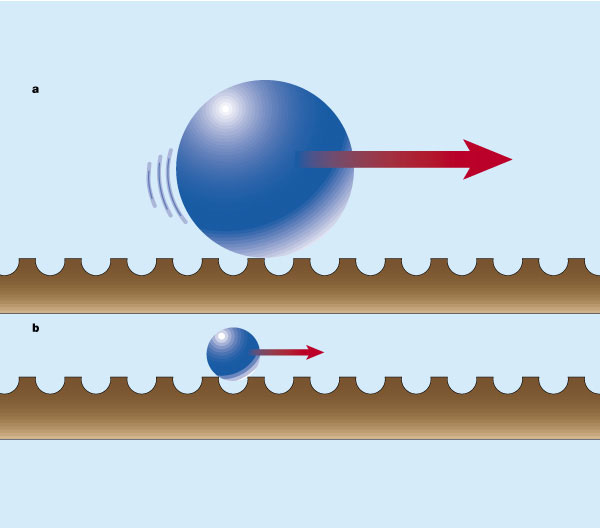
\includegraphics[width=0.6\textwidth,height=0.8\textheight]{Particles.jpg}
%    % Particles.jpg: 600x528 pixel, 100dpi, 15.24x13.41 cm, bb=0 0 432 380
% \end{center}
% 
% \caption{}
% \end{figure} 


\begin{figure}[!htb]
\centering
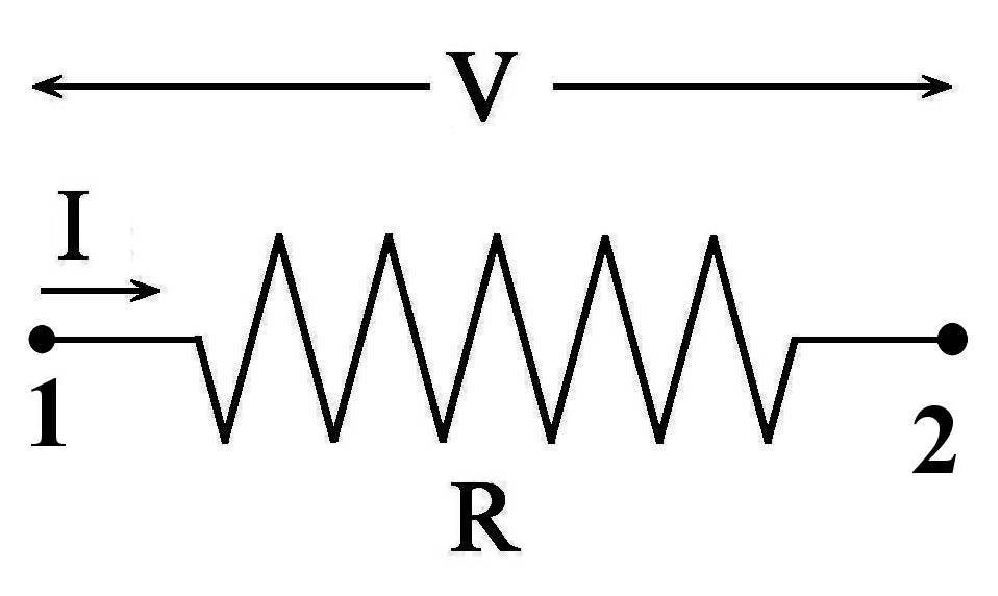
\includegraphics[width=0.70\linewidth]{Resistor_02.eps}
\caption{Resistor}
\label{fig:Resistor}
\end{figure}


Num resistor, há uma conversão de energia elétrica em energia
térmica, dada pelo efeito Joule. A potência dissipada pelo resistor
devido ao efeito Joule é dada por\cite{RLandau97,DeVries93}:
\begin{equation*}
P=RI^{2}=VI
\end{equation*}

\begin{equation}
M =
\begin{pmatrix}
1/a & x & x \\
-\cos\gamma/(a\sin\chi) & 2 & x \\
x & x & 3
\end{pmatrix}
\end{equation}

Na superfície da figura

\begin{figure}[!h]
\centering
\includegraphics[width=0.70\linewidth,angle=-90]{Superficie.eps}
\caption{Teste 2}
\label{Resistor}
\end{figure}

Este gráfico foi feito no gnuplot usando
o modo pm3d. Na equação de Scrodinger (\ref{eq:Sch})
ou \eqref{eq:Sch}

\begin{align}
   a & = f \\
   b & = s
\end{align}

%\setlength\arrayrulewidth{2pt}\arrayrulecolor{blue}
%\setlength\doublerulesep{2pt}\doublerulesepcolor{blue}
\begin{table}
\begin{center}
\begin{tabular}{c | c | c}
0 & 2 & 3\\ \hline
\rowcolor{cinza}\multicolumn{1}{c}{5} & \multicolumn{1}{c}{5} & \multicolumn{1}{c}{5} \\
\hline
\rowcolor[gray]{.8} 1 & 1 & 1\\
4 & 6 & 8
\end{tabular}
\end{center}
\end{table}



\section{Introdução}

O Método das Diferenças Finitas (MDF) é um método geralmente
utilizado para resolver equações diferenciais. Inicialmente
discretizamos o espaço, e esta discretização poderá ser
uniforme ou não e posteriormente reescrevemos a equação\cite[ver pag. 34]{RLandau97}
diferencial em termos das diferenças. Nos casos que iremos estudar
agora, iremos considerar uma discretização não uniforme,
conforme a figura ~\ref{fig2} abaixo.

\begin{equation}
   x^2\Longleftrightarrow
\end{equation} 

\begin{figure}[htb]
\centering
\setlength{\unitlength}{0.0040in}%
\begin{picture}(565,100)(15,450)
\thicklines
\put(150,480){\circle*{7}}
\put(170,480){\circle*{7}}
\put(190,480){\circle*{7}}
\put(415,480){\circle*{7}}
\put(435,480){\circle*{7}}
\put(455,480){\circle*{7}}
\put(-53,480){\line( 1, 0){185}}
\put(-60,480){\circle{15}}
%%\put(-60,490){\line( 0,-1){ 20}}
%%\put( 20,480){\line( 1, 0){100}}%%
%%\put( 20,490){\line( 0,-1){ 20}}
\put( 20,480){\circle*{15}}
\put( 20,470){\line( 0, 1){  0}}
%%\put(100,490){\line( 0,-1){ 20}}
\put(100,480){\circle*{15}}
\put(200,480){\line( 1, 0){200}}
\put(220,480){\circle*{15}}
\put(300,480){\circle*{15}}
\put(380,480){\circle*{15}}
\put(500,480){\circle*{15}}
\put(580,480){\circle*{15}}
%\put(220,490){\line( 0,-1){ 20}}
%\put(300,490){\line( 0,-1){ 20}}
%\put(380,490){\line( 0,-1){ 20}}
%\put(500,490){\line( 0,-1){ 20}}
%\put(580,490){\line( 0,-1){ 20}}
\put(480,480){\line( 1, 0){173}}
%\put(660,490){\line( 0,-1){ 20}}
\put(660,480){\circle{15}}
\put(225,500){\makebox(0,0)[lb]{\raisebox{0pt}[0pt][0pt]{ $\Delta x_{i-1}$}}}
\put(320,500){\makebox(0,0)[lb]{\raisebox{0pt}[0pt][0pt]{ $\Delta x_{i}$}}}
\put(-65,440){\makebox(0,0)[lb]{\raisebox{0pt}[0pt][0pt]{\large $0$}}}
\put( 15,440){\makebox(0,0)[lb]{\raisebox{0pt}[0pt][0pt]{\large $1$}}}
\put( 95,440){\makebox(0,0)[lb]{\raisebox{0pt}[0pt][0pt]{\large $2$}}}
\put(195,440){\makebox(0,0)[lb]{\raisebox{0pt}[0pt][0pt]{\large $i-1$}}}
\put(295,440){\makebox(0,0)[lb]{\raisebox{0pt}[0pt][0pt]{\large $i$}}}
\put(357,440){\makebox(0,0)[lb]{\raisebox{0pt}[0pt][0pt]{\large $i+1$}}}
\put(473,440){\makebox(0,0)[lb]{\raisebox{0pt}[0pt][0pt]{\large $n-1$}}}
\put(572,440){\makebox(0,0)[lb]{\raisebox{0pt}[0pt][0pt]{\large $n$}}}
\put(632,440){\makebox(0,0)[lb]{\raisebox{0pt}[0pt][0pt]{\large $n+1$}}}
%\put(247,490){\makebox(0,0)[lb]{\raisebox{0pt}[0pt][0pt]{\large $i-1$}}}
%\put(345,490){\makebox(0,0)[lb]{\raisebox{0pt}[0pt][0pt]{\large $i$}}}
\end{picture}
\vspace{-0.2cm}
\caption{Discretiza\c{c}\~{a}o da rede \label{fig2}}
\end{figure}%


Aqui iremos nos restringir a problemas em que temos equações
diferenciais de no máximo segunda ordem. Consideremos a expansão em 
série de Taylor da função $f(x)$ em torno do ponto $x_{i}$ (ver
figura ~\ref{fig2}). Na figura ~\ref{fig2} onde o índice $i$ indica um
ponto da rede discretizada, onde $f_{i}=f(x_{i})$ é o valor da 
função $f(x_{i})$ neste ponto e $\Delta _{i}=\Delta x_{i}=x_{i+1}-x_{i}$,
conforme mostra a figura~\ref{fig2}. Neste tipo de problema é muito
comum usarmos as seguintes condições de contorno: $f_{0}=f_{n+1}=0$,
$\Delta _{0}=\Delta _{1}$ e $\Delta _{n}=\Delta _{n-1}$.

\begin{align}
f(x+\Delta x_{i}) = & f(x) +\Delta x_{i}f^{\prime }(x) 
+\dfrac{\Delta x_{i}^{2}}{2!}f^{\prime \prime }(x) + \notag \\
& O(\Delta x_{i}^{3}) \label{df0}
\end{align}

\begin{align}
f(x+\Delta x_{i}) = & f(x)+\Delta x_{i}f^{\prime }(x)+
\dfrac{\Delta x_{i}^{2}}{2!}f^{\prime \prime }(x) + \notag \\ 
& O(\Delta x_{i}^{3})  \label{df1}
\end{align}

\begin{align}
f(x-\Delta x_{i-1}) = & f(x)-\Delta x_{i-1}f^{\prime }(x)+
\dfrac{\Delta x_{i-1}^{2}}{2!}f^{\prime \prime }(x) + \notag \\ 
& O(\Delta x_{i-1}^{3})  \label{df2}
\end{align}

\begin{align}
  & f(x+\Delta x_{i}) +f(x-\Delta x_{i-1}) \cong  2f(x) + \notag \\ 
  &\left( \Delta x_{i}-\Delta x_{i-1}\right) f^{\prime }(x) +
 \dfrac{(\Delta x_{i-1}^{2}+\Delta x_{i}^{2})}{2}f^{\prime \prime }(x)  
 \label{df3}
\end{align}

\begin{align}
  & f(x+\Delta x_{i}) - f(x-\Delta x_{i-1})  \cong  \notag \\ 
  & \left( \Delta x_{i-1} + \Delta x_{i} \right) f^{\prime }(x) -
 \dfrac{(\Delta x_{i-1}^{2}-\Delta x_{i}^{2})}{2} f^{\prime \prime }(x) \label{df4}
\end{align}
Podemos reescrever a eq. (\ref{df4}) como:

\begin{align}
f^{\prime }(x) & = \dfrac{f(x+\Delta x_{i})-f(x-\Delta x_{i-1})}{\Delta
x_{i-1}+\Delta x_{i}} - \notag \\ 
 & \dfrac{(\Delta x_{i}-\Delta x_{i-1})}{2}f^{\prime \prime }(x)  \label{df5}
\end{align}

Agora, substituindo a eq. (\ref{df5}) em (\ref{df3}), obtemos

\begin{equation}\label{edo1}
   \frac{{{d}^{2}}}{d{{t}^{2}}}\operatorname{x}(t)-6=0
\end{equation} 

\begin{footnotesize}
\begin{verbatim}
// Defina uma funcao f(i,x,y1,y2,..,ym) com i=1,2,..,m

// A solucao do sistema de  equações diferenciais: 

//      y1'= f(1,x,y1,y2,...,ym)

//      y2'= f(2,x,y1,y2,...,ym)

//      

//      ym'=f(m,x,y1,y2,...,ym)

//function R=f(i,x,y) // note que y pode ser passado como um vetor

//    select i

//    case 1 then

//        R=f1(x,y(1),y(2),...,y(m))   // defina a primeira função

//     case 2 then

//         R=f2(x,y(1),y(2),...,y(m))  // defina a segunda função

//         .

//         .

//         .

//     case m then

//         R=fm(xy(1),y(2),...,y(m)) // defina a m-esima função

//    end

//endfunction
\end{verbatim} 
\end{footnotesize}


% O estilos de referência se encontram no seguinte diretorio:
% /usr/share/texmf-texlive/bibtex/bst/

% O comando \nocite adiciona uma lista de referências sem que elas 
% necessitem de aparecer no texto.
\nocite{Franco2006,Heath1997,Davies-SciAm2006,Castro2001,Bolivar2001}

%Aqui faremos referências aos livros clássico do TeX e LaTeX


%\bibliographystyle{alpha}
%\bibliographystyle{unsrt}
% \bibliographystyle{abbrv}
% \bibliographystyle{apalike}
%\bibliographystyle{ieeetr}
%\bibliographystyle{siam}
\bibliographystyle{abntex2-num}
%\bibliographystyle{abntex2-alf}
%\bibliographystyle{apsrmp}
%\bibliographystyle{apsrev}
%\bibliographystyle{apsrev4-1}
%\bibliographystyle{MyUnsrt}
%\bibliographystyle{MyPlain}
%\bibliographystyle{MyPaper}
%\bibliographystyle{unsrt}

\bibliography{bibtex/FisComp_asc,bibtex/EnsinoPapers_asc}

\end{document}
